% !Mode:: "TeX:UTF-8:Main"
% arara: pdflatex
%needs ticksducks.sty from github!
\documentclass{article}
\usepackage[utf8]{inputenc} %probably not needed ...
\usepackage[T1]{fontenc}
\usepackage{geometry}
\geometry{papersize={128mm,96mm},margin=0.5cm} %\textwidth=11.8, \textheight=8.6
\usepackage[x11names,svgnames]{xcolor}
\usepackage{tikzducks}
\usetikzlibrary{shapes.geometric}
\usetikzlibrary{patterns}

\pagestyle{empty}
\parindent=0pt
\usepackage{animate}
\usepackage{eso-pic}
\usepackage{xfp}
\definecolor{mggreen}{RGB}{37,166,89}


\begin{document}
\AddToShipoutPictureBG{%
 \AtPageLowerLeft{%
 \begin{tikzpicture}[overlay,remember picture]
 \node[anchor=south west] at (7.5,2.6) {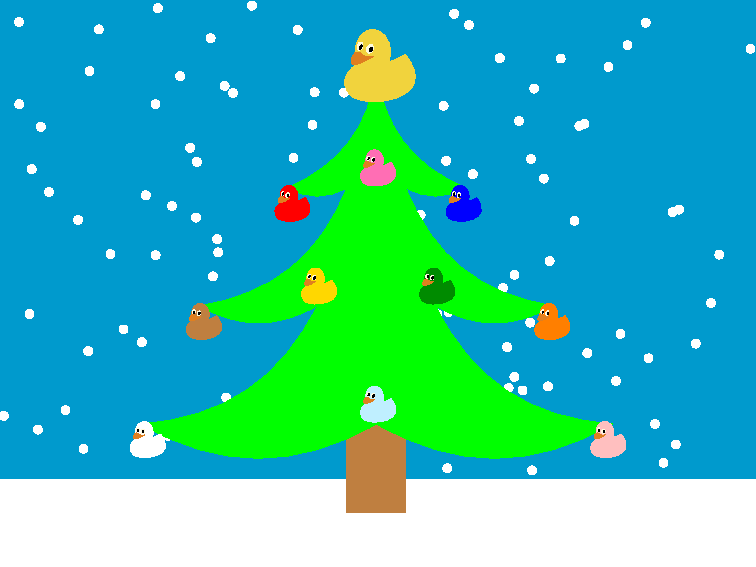
\includegraphics[width=0.7\textwidth]{prisoner_duck-background}};
 \fill[SlateGray4,even odd rule] (0,0) rectangle (\paperwidth,\paperheight) (9.5,5.5) rectangle (12,8.8) ;
 \fill[pattern=bricks,pattern color=SlateGray4!70!white,even odd rule] (0,0) rectangle (\paperwidth,\paperheight) (9.5,5.5) rectangle (12,8.8) ;
%
% \fill[LawnGreen] (0,0) rectangle (\paperwidth,\paperheight);
\draw[SlateGray4!70!black,thick] (9.5,5.5) rectangle (12,8.8) ;
\foreach\x in {1,2,...,5}
{
\draw[line width=1.5mm,SlateGray4!70!black](\fpeval{9.25+\x*0.5},5.5) --++(0,3.3);
}
 \end{tikzpicture}}}

\begin{tikzpicture}[]
\path (0,0) rectangle (\textwidth,\textheight);


\begin{scope}[xshift=3cm,yshift=1cm,scale=2.2]
\duck[crazyhair=gray!40!black,tshirt=white,stripes={
\stripes[rotate=100,color=gray!40!black]},prison=gray!60!black,grumpy,body=DarkGoldenrod1!20!AntiqueWhite1]
\end{scope}
\end{tikzpicture}

\end{document} 